\documentclass[a4paper,12pt]{article}

\usepackage{graphicx}
\usepackage{hyperref}
\usepackage[italian]{babel}
\usepackage{parskip}
\usepackage{multicol}
\usepackage{verbatim}
\usepackage[a4paper,left=2cm,right=2cm,top=2.5cm,bottom=2.5cm]{geometry}
\usepackage{float}
\usepackage{setspace}
\usepackage{svg}
\usepackage{amsmath}

\setlength{\parskip}{1em}
\graphicspath{ {./images/} }
\hypersetup {
    colorlinks=true,
    linkcolor=black,
    urlcolor=blue,
    citecolor=blue,
    pdfborderstyle={/S/U/W 1},
    }
\pagenumbering{gobble}
    \begin{document}
    \begin{titlepage}
        \begin{center}
            \begin{minipage}{0.3\textwidth}
                
\includegraphics[width=\linewidth]{Logo_Universita.png}
            \end{minipage}

        \end{center}

        \begin{center}
            \noindent\rule{0.7\textwidth}{0.4pt}\\[0.5cm]
            \large\textbf{Università degli Studi di Padova}\\
            \large Corso di Laurea in Informatica\\
            \small A. A. 2025/26
        \end{center}

        \vspace{1,5cm}    

    \begin{center}
        \begin{minipage}{0.5\textwidth}
            \includesvg[width=\linewidth]{logo}
        \end{minipage}
    \end{center}

        \vspace{1,5cm}    
        \begin{center}
            {\Large \textbf{Relazione}\par}
            \vspace{0.6cm}
            {\Large Progetto di Tecnologie Web\par}
            \vspace{0.3cm}
        \end{center}
        \vfill

        \centering
        \begin{tabular}{r|l}
            \textbf{Studenti} & Sofia De Blasi - 2111014 - \underline{\href{mailto:sofia.deblasi@studenti.unipd.it}{sofia.deblasi@studenti.unipd.it}}\\
             & Nicola Simionato - 2113190 - \underline{\href{mailto:nicola.simionato.5@studenti.unipd.it}{nicola.simionato.5@studenti.unipd.it}} \\
            & Nenad Radulovic - 2101059 - \underline{\href{mailto:nenad.radulovic@studenti.unipd.it}{nenad.radulovic@studenti.unipd.it}} \\
            & Giacomo Speggiorin - 2116438 - \underline{\href{mailto:giacomo.speggiorin@studenti.unipd.it}{giacomo.speggiorin@studenti.unipd.it}} \\
            & \\
            \textbf{Indirizzo del sito} & \underline{\url{https://tecweb.studenti.math.unipd.it/sdeblasi/}}\\
            & \\
            \textbf{Utente} & 
            \textbf{Username:} user, \textbf{Password:} user \\ 


        \end{tabular}

        \vfill

    \end{titlepage}     
    \newpage
    \tableofcontents
    \newpage
\clearpage 
\pagenumbering{arabic}
\section{Introduzione}

\subsection{Com'è nata l’idea}
L’idea del progetto nasce dall’esigenza, comune tra gli studenti universitari, di individuare rapidamente eventi, attività e servizi utili nella propria città universitaria. Attualmente tali informazioni risultano frammentate tra diversi canali (pagine social, bacheche fisiche sparse, etc.), rendendo la ricerca poco immediata.

Da questa osservazione è emersa la necessità di una piattaforma unica che centralizzi la pubblicazione di eventi e iniziative, permetta agli studenti di consultarli senza monitorare più fonti e offra agli organizzatori un punto di raccolta comune.

La riflessione si è estesa anche ad altri servizi rilevanti per la vita universitaria come ripetizioni, affitti e progetti sperimentali. Da qui l’idea di creare uno spazio organizzato, accessibile e pensato per raccogliere tutto ciò che può risultare utile nella quotidianità studentesca.

\section{Analisi del lavoro svolto}

\subsection{Processo decisionale}
Durante lo sviluppo del progetto sono state necessarie numerose decisioni riguardanti design, funzionalità e contenuti. La maggior parte delle scelte è stata discussa in presenza tra tutti i membri del gruppo, ma sono stati adottati anche canali sincroni e asincroni.

Per le comunicazioni asincrone è stata utilizzata la piattaforma di messaggistica 
\textbf{WhatsApp}, mentre 
\textbf{Discord} è stato impiegato come supporto alle riunioni e per la gestione delle comunicazioni sincrone a distanza.

\subsection{Modalità di lavoro}
Per garantire flessibilità organizzativa, il gruppo ha scelto una modalità di lavoro prevalentemente asincrona. 

Le attività sono state distribuite in modo che ciascun componente lavorasse su aspetti differenti, evitando sovrapposizioni. A supporto di questa organizzazione è stato adottato un sistema di versionamento tramite 
\textbf{Git} con hosting su 
\textbf{GitHub}, utile per tracciare modifiche, gestire branch e mantenere un flusso di lavoro ordinato.

\subsection{Divisione del lavoro}

Considerata la natura accademica del progetto, si è scelto di coinvolgere ogni membro del gruppo in tutte le principali aree di sviluppo, così da garantire una comprensione completa del funzionamento della piattaforma e una partecipazione equilibrata. 

La progettazione e la realizzazione del sito sono state quindi affrontate in modo collaborativo: tutti i componenti hanno contribuito alla struttura HTML, allo sviluppo dei fogli di stile, all’implementazione della logica PHP, alla progettazione del database, ai test di accessibilità e alla validazione lato client e lato server.

Per coordinare il lavoro sono state organizzate riunioni periodiche di allineamento e sono state utilizzate le \textbf{GitHub Issues}, che hanno permesso di tracciare in modo chiaro le attività, le priorità e lo stato di avanzamento, garantendo una distribuzione bilanciata dei compiti.

\subsection{Docker}

Per garantire un ambiente di sviluppo uniforme tra i membri del gruppo è stato utilizzato Docker.  
È stata predisposta un’immagine contenente:

\begin{itemize}
    \item un database \textbf{MariaDB} (v. 10.6.7);
    \item un server \textbf{Apache PHP} (v. 8.2);
    \item un’istanza di \textbf{phpMyAdmin}.
\end{itemize}

Questa configurazione ha permesso di evitare differenze tra sistemi operativi, velocizzare il lavoro 
e avviare tutti i servizi necessari tramite un unico \texttt{docker-compose}.

\section{Progettazione}
\subsection{Analisi dei contenuti}

La piattaforma funge da bacheca universitaria online, articolata in quattro categorie principali: 
\textbf{Affitti}, \textbf{Esperimenti}, \textbf{Eventi} e \textbf{Ripetizioni}. Ogni annuncio condivide una struttura comune, 
arricchita da attributi specifici in base alla categoria.

\paragraph{Campi generici}
Ogni annuncio contiene:
\begin{itemize}
    \item \textbf{Categoria} (una delle quattro disponibili);
    \item \textbf{Titolo} e \textbf{Descrizione};
    \item \textbf{Data di pubblicazione} (generata automaticamente);
    \item \textbf{Città} di riferimento;
    \item \textbf{Autore} (utente registrato).
\end{itemize}

\paragraph{Campi specifici}
Ogni categoria prevede tre attributi dedicati:
\begin{multicols}{2}
\begin{itemize}
    \item \textbf{Affitti}: prezzo mensile, indirizzo, numero coinquilini.
    \item \textbf{Esperimenti}: laboratorio, durata prevista, compenso.
    \item \textbf{Eventi}: data, luogo, costo entrata.
    \item \textbf{Ripetizioni}: materia, livello, prezzo orario.
\end{itemize}
\end{multicols}

\subsection{Descrizione delle funzionalità}

\paragraph{Registrazione e accesso}
Gli utenti possono registrarsi tramite un form dedicato e accedere alle funzionalità riservate.

\paragraph{Pubblicazione e gestione annunci}
Gli utenti autenticati possono creare, modificare ed eliminare i propri annunci.  
Gli annunci eliminati vengono rimossi anche dalle liste dei preferiti.

\paragraph{Ricerca e filtraggio}
Il sistema offre: \textbf{filtri generici} (categoria, data), \textbf{filtri specifici} per categoria e \textbf{ricerca testuale} su titolo, descrizione ed email dell’autore.

\paragraph{Validazione}
Nei form con attributo \texttt{data-validate}, l’invio viene bloccato in caso di dati non validi.  
La validazione è gestita sia lato client sia lato server (si veda \underline{\hyperref[sviluppo:validazione]{la sezione sulla validazione}}).

\subsection{Architettura del sistema}

Il progetto segue una chiara separazione tra: \textbf{struttura} (HTML), \textbf{presentazione} (CSS), \textbf{comportamento} (JavaScript), \textbf{logica applicativa} (PHP) e \textbf{persistenza} (database).

La composizione delle pagine avviene tramite template HTML presenti in \textbf{/pages}, 
nei quali PHP inserisce dinamicamente i contenuti.  
Le risorse statiche sono organizzate in cartelle dedicate (\textbf{/css}, \textbf{/js}, \textbf{/assets}, \textbf{/img\_annunci}).

\subsection{Struttura del sito}

La struttura del sito è stata analizzata tramite un modello ad albero (vedi~Figura~\ref{fig:albero}), utile per valutarne ampiezza e profondità ed evidenziare i percorsi di navigazione principali.

\begin{figure}[H]
    \centering
    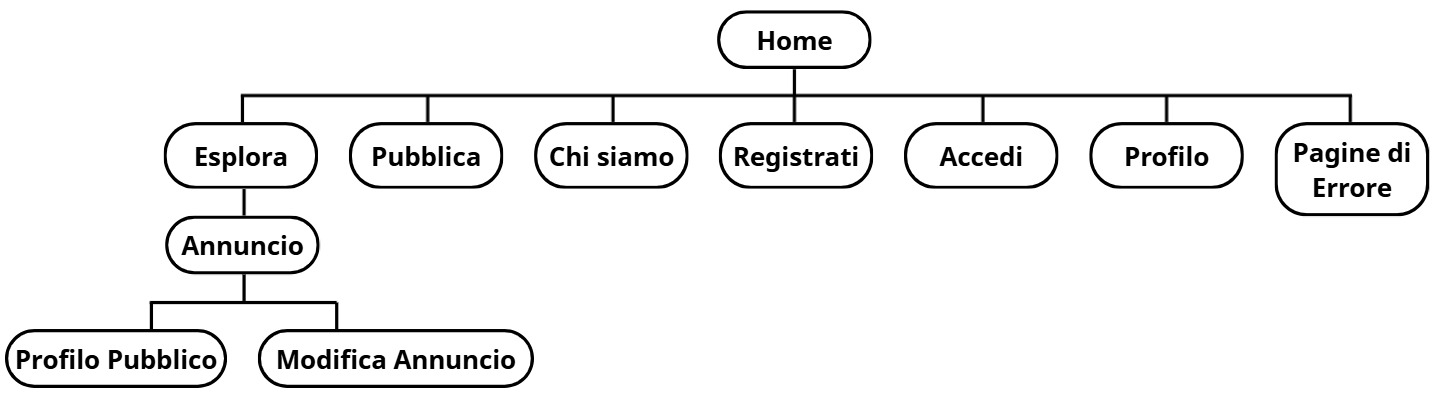
\includegraphics[width=1\textwidth]{albero_sito.png}
    \caption{Rappresentazione ad albero della struttura del sito}
    \label{fig:albero}
\end{figure}

Dal punto di vista dell’architettura dell’informazione, il sito presenta una \textbf{ampiezza (7) maggiore rispetto alla profondità (4)}: le funzionalità principali sono raggiungibili direttamente dalla homepage o con al massimo tre livelli di navigazione. Questa scelta riduce il carico cognitivo e facilita l’orientamento, soprattutto per utenti alla prima visita.

\subsection{Schema di navigazione e metafora della pesca}
La navigazione del sito combina struttura gerarchica e percorsi trasversali, richiamando la 
\textbf{metafora della pesca} per rappresentare i diversi modi in cui l’utente può ricercare i contenuti:
\begin{itemize}
    \item \textbf{Barra di ricerca} $\rightarrow$ \emph{tiro perfetto}: permette di individuare rapidamente un annuncio specifico.
    \item \textbf{Filtri generici e specifici} $\rightarrow$ \emph{trappola per aragoste}: restringono progressivamente il campo dei risultati.
    \item \textbf{Accesso diretto alle categorie} $\rightarrow$ \emph{pesca con la rete}: consente di esplorare insiemi omogenei di contenuti.
    \item \textbf{Ultimi annunci inseriti} $\rightarrow$ \emph{pesca con la rete}: favorisce la scoperta casuale.
    \item \textbf{Preferiti e area personale} $\rightarrow$ \emph{boa di segnalazione}: permette di raccogliere e ritrovare facilmente i contenuti di interesse.
\end{itemize}

\subsection{Pagine di errore}
Ogni errore è stato progettato per non essere bloccante: sono sempre presenti elementi di interazione chiari, come il pulsante per tornare alla \emph{Home} o il collegamento diretto alla bacheca degli annunci. Questo permette all’utente di recuperare rapidamente la navigazione senza sentirsi “intrappolato” nella pagina di errore. Inoltre, abbiamo scelto di utilizzare un tono leggero e leggermente ironico.
La gestione degli errori viene effettuata sia tramite codice PHP restituendo la pagina personalizzata relativa all'errore specifico che attraverso il
file .htaccess che reindirizza gli errori a pagine personalizzate.


\subsection{Database}

Il database è stato progettato per essere semplice, normalizzato e facilmente estendibile, 
in linea con le esigenze di una bacheca universitaria.  
Le entità principali sono: \textbf{Utente}, \textbf{Città}, \textbf{Annuncio}, le quattro 
\textbf{specializzazioni di Annuncio}, \textbf{ImmaginiAnnuncio} e \textbf{Preferiti}.

\paragraph{Schema ER}

La figura (vedi~Figura~\ref{fig:ER}) mostra il modello concettuale, in cui \texttt{Annuncio} rappresenta 
l’entità centrale e viene estesa da quattro specializzazioni, una per ciascuna categoria 
(\textbf{Affitti}, \textbf{Esperimenti}, \textbf{Eventi}, \textbf{Ripetizioni}).  
Ogni specializzazione aggiunge tre attributi specifici, evitando duplicazioni nei campi generici.

\paragraph{Ristrutturazione della generalizzazione}
In fase logica, la generalizzazione è stata trasformata in quattro relazioni \texttt{IS-[categoria]}, 
ciascuna collegata a \texttt{Annuncio} tramite chiave primaria condivisa (vedi~Figura~\ref{fig:ERristrutturato}).  
Questa scelta mantiene la normalizzazione e semplifica l’estendibilità del modello.

\begin{figure}[h!]
    \centering
    \begin{minipage}{0.48\textwidth}
        \centering
        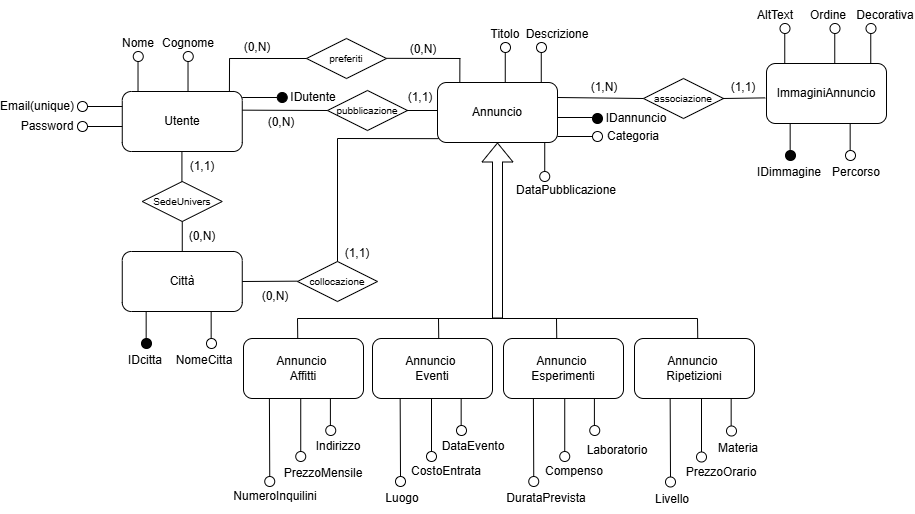
\includegraphics[width=\textwidth]{ER.png}
        \caption{Schema ER}
        \label{fig:ER}
    \end{minipage}
    \hfill
    \begin{minipage}{0.48\textwidth}
        \centering
        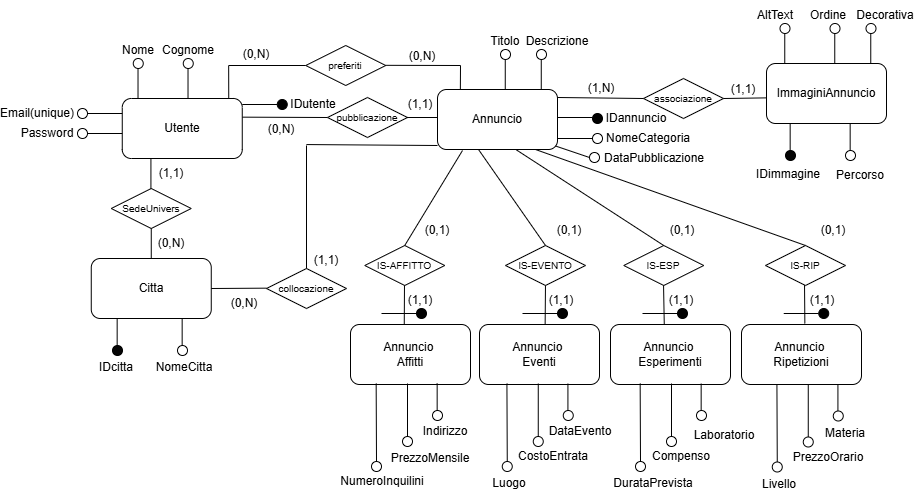
\includegraphics[width=\textwidth]{ERristrutturato.png}
        \caption{Schema ER ristrutturato}
        \label{fig:ERristrutturato}
    \end{minipage}
\end{figure}

\paragraph{Schema relazionale}
Le tabelle principali sono:

\begin{itemize}
    \item \textbf{Utente}(\underline{IdUtente}, Nome, Cognome, Email [UNIQUE], Password, IdCittà*)
    \item \textbf{Città}(\underline{Idcittà}, Nomecittà [UNIQUE])
    \item \textbf{Annuncio}(\underline{IdAnnuncio}, Titolo, Descrizione, DataPubblicazione, Idutente, Categoria, IdCittà)
    \item \textbf{Affitti}(\underline{IdAnnuncio}, PrezzoMensile, Indirizzo, NumeroInquilini)
    \item \textbf{Esperimenti}(\underline{IdAnnuncio}, Laboratorio, DurataPrevists, Compenso)
    \item \textbf{Eventi}(\underline{IdAnnuncio}, DataEvento, Luogo, CostoEntrata)
    \item \textbf{Ripetizioni}(\underline{IdAnnuncio}, Materia, Livello, PrezzoOrario)
    \item \textbf{ImmaginiAnnuncio}(\underline{IdImmagine}, IdAnnuncio, Percorso, AltText*, Decorativa, Ordine)
    \item \textbf{Preferiti}(\underline{IdAnnuncio}, \underline{IdUtente})[UNIQUE]
\end{itemize}

Le relazioni sono collegate tramite chiavi esterne con vincoli \texttt{ON DELETE CASCADE} 
nelle tabelle dipendenti (specializzazioni, immagini, preferiti), così da mantenere la coerenza 
dei dati in caso di eliminazione di un annuncio.

\paragraph{Normalizzazione}
Lo schema rispetta la 3NF:
\begin{itemize}
    \item attributi atomici (1NF);
    \item dipendenza completa dalla chiave primaria nelle specializzazioni (2NF);
    \item assenza di dipendenze transitive (3NF).
\end{itemize}

\paragraph{Scelte progettuali}
Sono stati adottati ID numerici auto-incrementali per garantire stabilità, efficienza nelle join 
e uniformità dello schema.  
La separazione tra \texttt{Annuncio} e le sue specializzazioni consente di aggiungere nuove categorie 
senza modificare la struttura esistente.

\section{Sviluppo}
\subsection{HTML}

Ogni documento è organizzato nelle sezioni \texttt{<head>} e \texttt{<body>}, con uso coerente di elementi semantici ed evitando tag puramente presentazionali.

\subsubsection{Meta tag \texttt{viewport}}
È stato inserito il meta tag:
\texttt{<meta name="viewport" content="width=device-width"/>}
che consente ai CSS di riferirsi alla larghezza effettiva del dispositivo, evitando l’applicazione del layout desktop su schermi ad alta densità di pixel.

\subsubsection{\texttt{<aside>} in \texttt{esplora.html}}
Nella pagina \texttt{esplora.html} l’elemento \texttt{<aside>} contiene i filtri di ricerca, poiché rappresentano contenuti accessori rispetto al flusso principale (lista degli annunci). 
Essendo una funzionalità secondaria all'interno della pagina sono stati adottati alcuni compromessi con JavaScript per accessibilità e usabilità.
In particolare, con la disattivazione di JavaScript, da telefono non è possibile aprire i filtri, che diventano una tendina laterale, su desktop invece rimanendo sempre
visibili non possono essere raggiunti tramite il tab, questo a causa dell'uso dell'attributo \texttt{inert}.

\subsubsection{Struttura di \texttt{cardTemplate}}
Le card degli annunci (\texttt{cardTemplate.html}) utilizzano \texttt{<h3>} per i titoli, evitando coppie \texttt{<dt>}–\texttt{<dd>}.  
La gerarchia semantica è così preservata: \texttt{<h2>} identifica la sezione (es. “Ultimi inseriti”), mentre \texttt{<h3>} rappresenta ciascun annuncio. 

\subsubsection{Gestione delle immagini}
La gestione delle immagini è progettata per ottimizzare prestazioni e accessibilità.

\begin{itemize}
    \item Le immagini above-the-fold usano \texttt{loading="eager"}, tutte le altre \texttt{loading="lazy"}.
    \item Formati adottati: WebP per immagini decorative, SVG per il logo e JPG per le immagini degli annunci.
    \item Tutte le immagini sono inferiori a 1 MB.
\end{itemize}

Le immagini decorative sono inserite nel markup e dimensionate via CSS; il logo utilizza tecniche di image replacement per mantenere accessibile il testo alternativo, mentre le immagini degli annunci hanno dimensioni fissate via HTML per rendere 
l'esperienza utente migliore in quanto ciò garantisce un rendering più veloce.

Nel form di pubblicazione/modifica l’utente deve rispettare vincoli espliciti (max 1 MB, formato JPG), infatti è presente un controllo sulla dimensione dei file.

Si è scelto di limitare i MIME type accettati, rinunciando a conversioni automatiche o all'utilizzo del tag \texttt{<picture>} con doppia estensione \texttt{.png} per la stampa e \texttt{.jpg} per il web, per privilegiare semplicità e controllo.

La gestione dell’attributo \texttt{alt} è affidata all’utente: ogni immagine deve avere un testo alternativo oppure essere marcata come decorativa, e non è possibile lasciare entrambi i campi vuoti. Il testo alternativo è limitato a 100 caratteri per garantire sintesi e usabilità con screen reader.

\subsubsection{Form e validazione}
La struttura dei form utilizza \texttt{fieldset} e \texttt{legend}, anche quando destinati principalmente alle tecnologie assistive, questo fa sì che nessun campo sia figlio diretto di \texttt{form}.  

Ogni input utilizza il tipo HTML più appropriato ed è sempre associato a una \texttt{label}. Dove utile, sono abilitati \texttt{autocomplete} e \texttt{spellcheck} adeguati.

La validazione sfrutta: controlli HTML5 (\texttt{required}, \texttt{min}, \texttt{max}, \texttt{step}, vincoli di tipo), validazione JavaScript per feedback più dettagliati ed istantanei e validazione lato server per garantire correttezza e sicurezza.

\subsubsection{Messaggio informativo nei redirect verso la pagina di accesso}
Quando l’utente viene reindirizzato alla pagina di accesso a seguito del tentativo di accedere a una funzionalità riservata, viene mostrato automaticamente un riquadro informativo
che spiega il motivo del redirect, con un messaggio contestuale alla pagina di provenienza (pubblicazione, modifica, profilo o salvataggio nei preferiti).

\subsection{CSS e decisioni di design}

I fogli di stile sono stati progettati privilegiando l’uso di dimensioni relative, così da garantire un’interfaccia adattabile a dispositivi e contesti differenti.

Per assicurare uniformità grafica è stata definita una \texttt{:root} contenente variabili CSS per colori, spaziature, raggi di arrotondamento, ombre, transizioni e una scala tipografica coerente per dimensioni e pesi dei caratteri.

Il layout è realizzato principalmente tramite Flexbox, utilizzato per strutture fluide e adattive, mentre CSS Grid è impiegato solo nei casi in cui risulta più appropriato (ad esempio per elenchi di card o sezioni a griglia).

La responsività è gestita tramite la separazione tra \texttt{style.css} e \texttt{mini.css}, con un breakpoint principale a 800px per l’adattamento ai dispositivi mobili. Sono presenti due ulteriori media query, tra cui una dedicata alla navigazione con menù hamburger, attivata sotto i 1000px per migliorare l’usabilità su tablet e schermi intermedi.

È stato inoltre previsto un foglio di stile dedicato alla stampa \texttt{print.css}, che mostra esclusivamente le informazioni essenziali, rimuovendo elementi decorativi e interattivi per ridurre il consumo di inchiostro ma mantenendo una struttura coerente del contenuto per evitare il fenomeno del disorientamento.

Particolare attenzione è stata riservata all’accessibilità visiva e all’interazione da tastiera, con la gestione esplicita degli stati di focus visibile, l’uso coerente dei contrasti e l’eliminazione di animazioni superflue nei contesti in cui potrebbero risultare problematiche, come nelle versioni mobile o di stampa.

\subsection{PHP}
Per consentire al sistema di generare pagine web il cui contenuto non sia statico,
ma vari in base al contesto, tutte le pagine vengono composte dinamicamente tramite PHP.
All'interno della cartella \textbf{/pages} sono presenti i template HTML, nei quali sono stati
inseriti marcatori racchiusi tra parentesi quadrate (ad esempio \textbf{[TitoloAnnuncio]}) che vengono sostituiti a runtime con i contenuti dinamici appropriati.

Oltre alla generazione delle pagine, il PHP si occupa di:
\begin{itemize}
    \item gestire tutte le richieste provenienti dal client tramite form;
    \item validare gli input dell'utente (si veda \underline{\hyperref[sviluppo:validazione]{la sezione sulla validazione}});
    \item gestire le sessioni di accesso dell'utente;
    \item reindirizzare l'utente non autenticato verso la pagina di accesso qualora tenti di raggiungere funzionalità riservate;
    \item reindirizzare la navigazione verso le pagine di errore in caso di condizioni inattese;
    \item gestire le connessioni al database, garantendo che non rimangano aperte più del necessario, e costruire correttamente le query.
          A tale scopo, tutte le operazioni relative al database sono state centralizzate nel file \textbf{dbConnect.php}, così da mantenere una chiara separazione del codice.
\end{itemize}

Per semplificare lo sviluppo e aumentare la riutilizzabilità del codice, è stata inoltre realizzata
una libreria interna al progetto, contenuta nel file \textbf{tool.php}.

\section{Accessibilità}

\subsection{Strumenti di verifica}

Sono stati utilizzati diversi strumenti di verifica:
\begin{itemize}
    \item \textbf{NVDA}: per testare la gerarchia dei titoli, la lista dei link e dei punti di riferimento, la navigazione tramite landmark e l’annuncio dei messaggi di errore nei form, sia con JavaScript attivo che disattivato (vedi Figure~\ref{fig:NVDA1} e~\ref{fig:NVDA2}).
\end{itemize}

\begin{figure}[h!]
    \centering
    \begin{minipage}{0.48\textwidth}
        \centering
        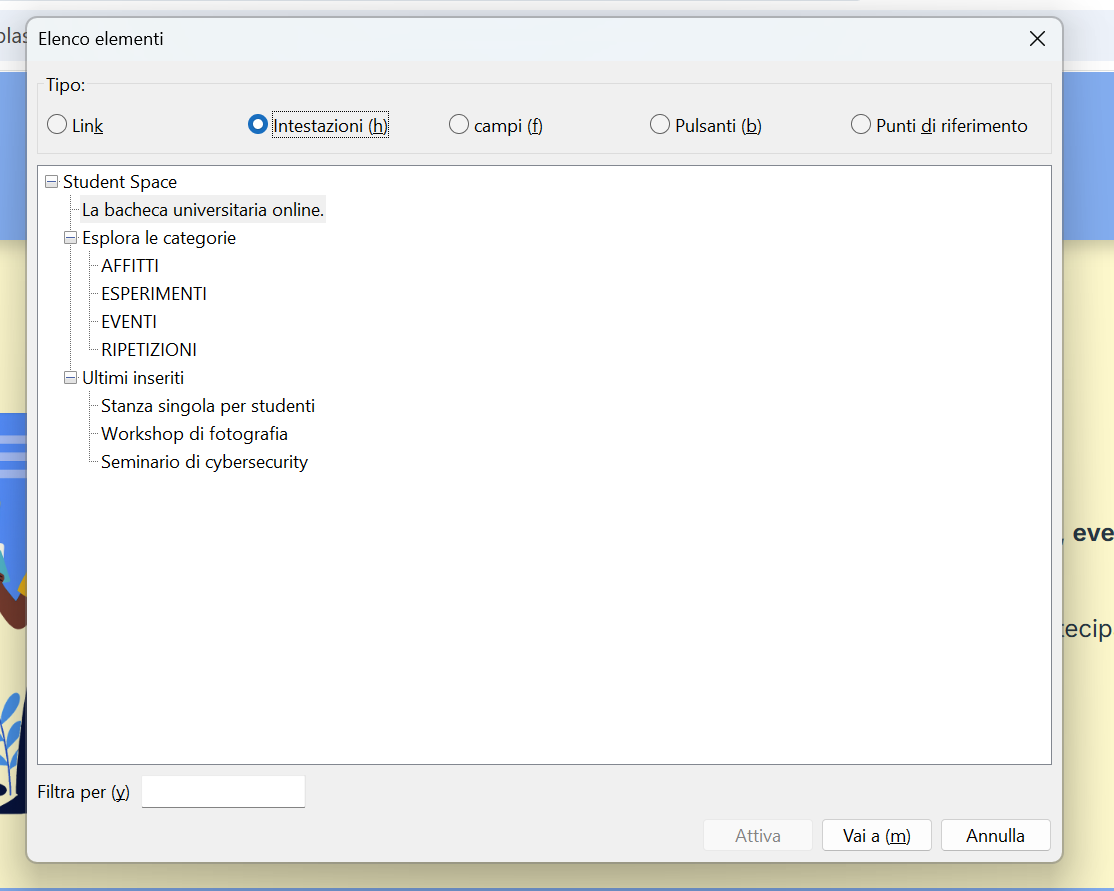
\includegraphics[width=\textwidth]{headings_index.png}
        \caption{Gerarchia dei titoli (index.html)}
        \label{fig:NVDA1}
    \end{minipage}
    \hfill
    \begin{minipage}{0.48\textwidth}
        \centering
        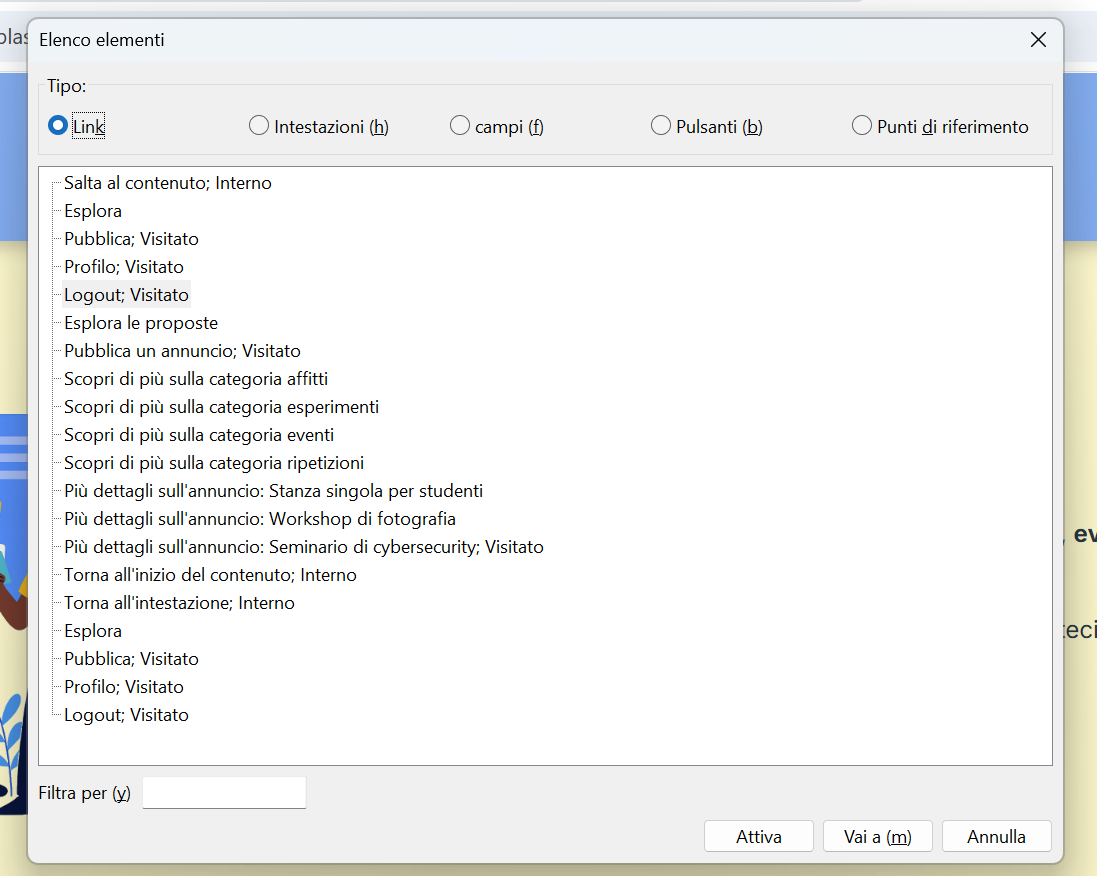
\includegraphics[width=\textwidth]{link_index.png}
        \caption{Lista dei link (index.html)}
        \label{fig:NVDA2}
    \end{minipage}
\end{figure}

\begin{itemize}
    \item \textbf{Contrast Checker} (\underline{\url{https://contrastchecker.com/}}): per verificare il rispetto del rapporto di contrasto $\geq 4.5\!:\!1$.
    \item \textbf{Lighthouse, Silktide e strumenti di ispezione (F12)}: per valutazioni automatiche e test manuali su navigazione da tastiera, accessibilità dei link, dimensioni degli elementi cliccabili e altri criteri WCAG.
\end{itemize}

\subsection{Tipografia e leggibilità}

Per garantire una lettura chiara e accessibile sono stati scelti due font distinti:

\begin{itemize}
    \item \textbf{Web}: \emph{Noto Sans}, importato tramite Google Fonts.
    \item \textbf{Stampa}: \emph{Times New Roman}.
\end{itemize}

La scelta del font web è stata guidata da verifiche sulla leggibilità di caratteri critici (\texttt{qp, db, 0O, iI1l, rn, m}), sull’altezza della \emph{x} e  sull'apertura delle lettere \emph{c} e \emph{a}.  
Inizialmente era stato considerato \texttt{Inter}, poi sostituito da \texttt{Noto Sans} per una migliore distinzione di glifi come \texttt{ca} e \texttt{iI1l} (vedi Figure~\ref{fig:font1} e~\ref{fig:font2}).

\begin{figure}[h!]
    \centering
    \begin{minipage}{0.48\textwidth}
        \centering
        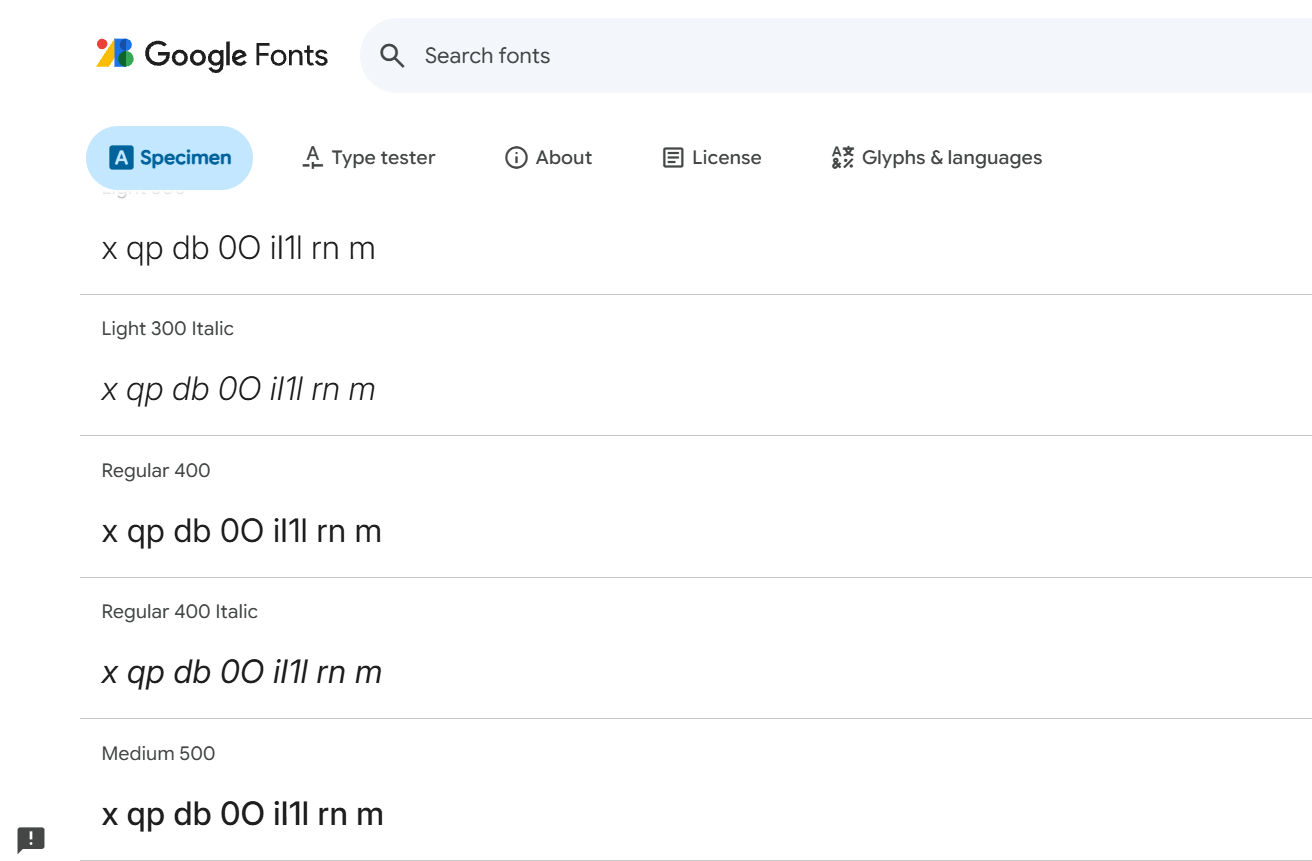
\includegraphics[width=\textwidth]{inter.png}
        \caption{Font: Inter}
        \label{fig:font1}
    \end{minipage}
    \hfill
    \begin{minipage}{0.48\textwidth}
        \centering
        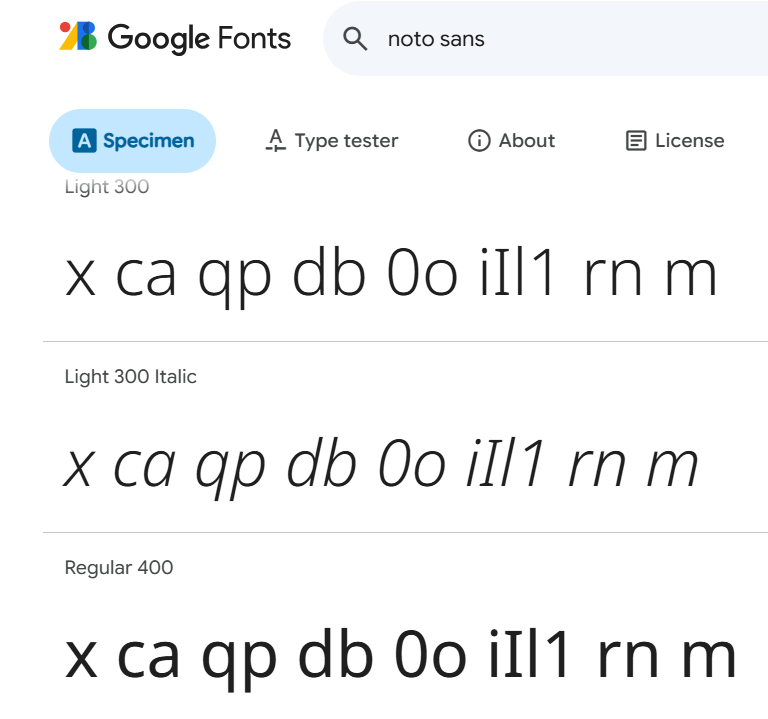
\includegraphics[width=\textwidth]{noto.png}
        \caption{Font: Noto Sans}
        \label{fig:font2}
    \end{minipage}
\end{figure}

\paragraph{Leggibilità dei prezzi}
La funzione PHP \texttt{Tool::formatPrezzo()} formatta i valori numerici mostrando i decimali solo quando necessario (es. \texttt{20€} invece di \texttt{20.00€}), migliorando la leggibilità.

\subsection{Colori, contrasti e accessibilità mobile}

Sono stati adottati diversi accorgimenti per garantire una corretta percezione dei contenuti e la riconoscibilità degli elementi interattivi:

\begin{itemize}
    \item \textbf{Link e Call To Action (CTA)}:
    \begin{itemize}
        \item I link testuali sono sempre sottolineati.
        \item I link visitati/non visitati nella navbar e nelle card annunci differiscono per colore (contrasto 2.72 $\approx 3$) mentre nelle card di categoria il colore del \texttt{:visited} è associato al colore della categoria con contrasto $\geq 3$.
        \item I pulsanti CTA variano colore tra stato visitato e non visitato (in \texttt{background-color} e \texttt{color}).
    \end{itemize}
    (\href{https://tecweb.studenti.math.unipd.it/sdeblasi/relazione/sommario-contrasti.pdf}{\underline{Apri il Sommario dei Contrasti} }(PDF, 34 KB))


    \item \textbf{Accessibilità touch su mobile}:
    \begin{itemize}
        \item Gli elementi cliccabili rispettano dimensioni minime di circa 44px × 44px.
        \item Il pannello laterale dei filtri utilizza un overlay e una gestione del focus accessibile (\texttt{toggleFiltriAccessibile()}).
        \item I pulsanti dei caroselli hanno opacità testata e leggibile (\texttt{rgba(22, 40, 110, 0.65)}).
    \end{itemize}
\end{itemize}

\begin{figure}[h!]
    \centering
    \begin{minipage}{0.48\textwidth}
        \centering
        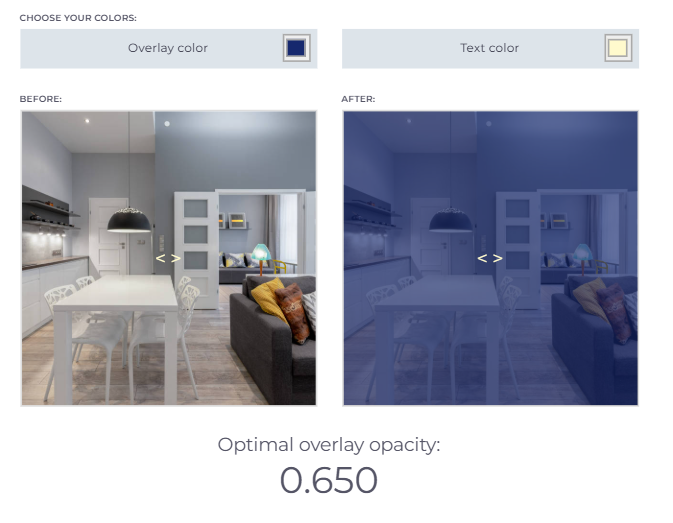
\includegraphics[width=0.7\textwidth]{opacita1.png}
        \caption{Opacità su immagine prova 1}
    \end{minipage}
    \hfill
    \begin{minipage}{0.48\textwidth}
        \centering
        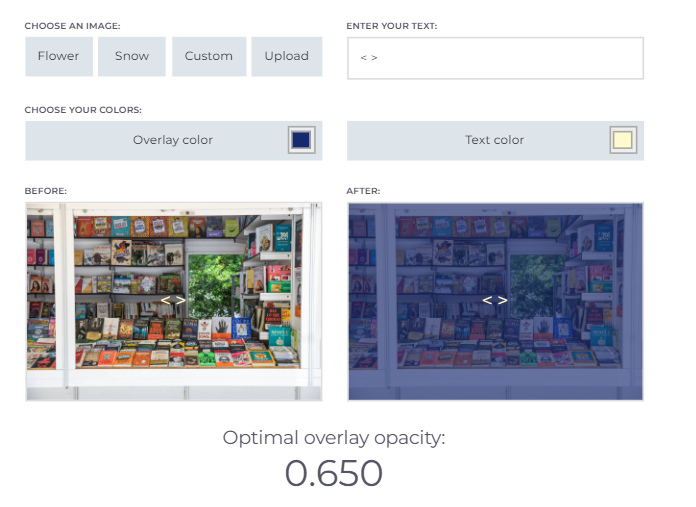
\includegraphics[width=0.7\textwidth]{opacita2.png}
        \caption{Opacità su immagine prova 2}
    \end{minipage}
\end{figure}

\section{Validazione, sicurezza e gestione degli errori}
\label{sviluppo:validazione}

\subsection{Errori lato client (JavaScript)}

La validazione lato client fornisce un feedback immediato all’utente, migliorando l’usabilità e riducendo il numero di richieste non valide inviate al server.  
Il comportamento è attivo esclusivamente nei form che dichiarano l’attributo \texttt{data-validate}, così da evitare interferenze con form che non richiedono controlli avanzati e immediati (pre-submit).

\paragraph{Gestione del focus}
All’avvio della pagina, lo script verifica la presenza di eventuali errori generati lato server:
\begin{itemize}
    \item in caso di errori relativi alle immagini, il focus viene portato sul primo input \texttt{file};
    \item in caso di errori su campi testuali, il focus viene portato sul primo campo non valido;
    \item quando un errore compare per la prima volta, il contenuto del campo viene selezionato per facilitare la correzione. E' stato deciso di riportare il focus sull'input errato solo la prima volta per evitare di essere troppo restrittivi.
\end{itemize}

\paragraph{Eventi di validazione}
La validazione viene eseguita in tre momenti distinti:
\begin{itemize}
    \item \textbf{blur}: quando un campo perde il focus, viene validato se ritenuto “validabile”;
    \item \textbf{input}: la digitazione rimuove eventuali messaggi di errore e ripristina gli attributi ARIA;
    \item \textbf{submit}: tutti i campi vengono validati; se uno o più risultano non validi, l’invio viene bloccato e il focus viene portato sul primo errore.
\end{itemize}

\paragraph{Criteri di validazione}
La funzione \texttt{validateField()} applica controlli specifici in base all’ID del campo: nome, cognome, email, password, confermaPassword, città (deve corrispondere a un valore presente nella lista \texttt{datalist}), consenso-email (deve essere selezionato).

Alcuni campi vengono esclusi dalla validazione client-side: input \texttt{file}, campi relativi al testo alternativo delle immagini (\texttt{alt}), campi relativi alla marcatura decorativa (\texttt{decorativa}).

\paragraph{Rendering degli errori}
Gli errori vengono mostrati tramite:
\begin{itemize}
    \item un contenitore \texttt{<ul>} con classi \texttt{riquadro-spieg} e \texttt{messaggi-errore-form};
    \item elementi \texttt{<li>} con classe \texttt{msgErrore} e \texttt{role="alert"};
    \item associazione dinamica di \texttt{aria-invalid="true"} e \texttt{aria-describedby}.
\end{itemize}

La funzione \texttt{removeError()} rimuove: il contenitore degli errori. l’attributo \texttt{aria-invalid} e eventuali riferimenti a messaggi non più presenti in \texttt{aria-describedby}.

\subsection{Errori lato server (PHP)}

La validazione lato server garantisce la corretta gestione degli input anche in assenza di JavaScript, assicurando coerenza, sicurezza e un comportamento uniforme in tutte le condizioni di utilizzo.

\begin{itemize}
    \item \textbf{Tipologie di errori}: campi generici, immagini (dimensione, formato, testo alternativo), credenziali di accesso.
    \item \textbf{Messaggi}: generati come liste con \texttt{role="alert"}, mantenendo la stessa struttura, semantica e classi CSS dei messaggi lato client.
    \item \textbf{Attributi ARIA}: applicazione dinamica di \texttt{aria-invalid} e \texttt{aria-describedby} ai campi non validi, con rimozione automatica quando l’errore viene risolto.
    \item \textbf{Gestione del focus}: il focus viene portato automaticamente sul primo campo non valido; nel caso delle immagini, sul primo input \texttt{file}. Quando appropriato, il contenuto del campo viene anche selezionato per facilitare la correzione.
    \item \textbf{Errori relativi alle immagini}: controllo della dimensione (1 MB), dei formati consentiti lato server (JPG, PNG, WEBP) e dell’obbligatorietà del testo alternativo. I form accettano solo JPG per semplicità, mentre il server gestisce anche PNG e WEBP per maggiore robustezza.
    \item \textbf{Login}: gestione degli errori di autenticazione tramite messaggi contestuali e sistema di \texttt{redirectMessage}, che informa l’utente del motivo del reindirizzamento.
\end{itemize}

Per motivi di sicurezza, nel processo di sanificazione degli input è stata adottata la funzione \texttt{strip\_tags()}, che rimuove i tag HTML e PHP dalle stringhe inserite dall’utente, prevenendo l’inserimento di codice malevolo.  

La funzione elimina i tag ma non il contenuto testuale: ad esempio, da \texttt{<strong>Descrizione evento...</strong>} vengono rimossi i tag \texttt{<strong>} e \texttt{</strong>}, mantenendo il testo interno. I tag in linea e i relativi attributi vengono invece completamente eliminati.

È stata valutata la possibilità di introdurre un controllo esplicito che segnalasse all’utente la presenza di tag HTML non consentiti. Tuttavia, nel sito sono presenti campi di input per i quali non sono previsti messaggi di errore dedicati.  
Per mantenere coerenza nella gestione dei feedback e dei controlli, si è scelto di applicare la sanificazione a tutti i campi senza generare errori specifici.

In questo modo:
\begin{itemize}
    \item se l’utente inserisce tag con intento semantico, il contenuto viene preservato e i tag rimossi;
    \item se l’input contiene un uso massiccio o sospetto di markup, viene comunque neutralizzato, assumendo che si tratti di un tentativo malevolo, considerando anche il target non tecnico della piattaforma.
\end{itemize}

\subsection{Sicurezza delle password}
Per garantire la sicurezza delle password degli utenti nella loro memorizzazione nel database, si è deciso di implementare un sistema di hashing delle password.
In particolare, si è scelto di appoggiarsi alla funzione nativa di PHP \texttt{password\_hash()}, che utilizza l'algoritmo BCRYPT per l'hashing delle password.

\section{Configurazione .htaccess} 
Il file \texttt{.htaccess} è un file di configurazione per il server web Apache, che nel nostro caso viene utilizzato per la sicurezza di alcune aree,
la gestione degli errori e per rendere più leggibili gli URL.
\begin{itemize}
    \item \textbf{Protezione aree riservate}: l'unico file ritenuto necessario da proteggere è stato il file \texttt{.env} che contiene le credenziali di accesso al database.
    \item \textbf{Gestione errori personalizzata}: il file .htaccess reindirizza gli errori 403, 404 e 500 a pagine di errore personalizzate (\texttt{403.php}, \texttt{404.php} e \texttt{500.php}).
    \item \textbf{URL rewriting}: il file .htaccess utilizza mod\_rewrite per creare URL più leggibili e SEO-friendly, rimuovendo estensioni come .php dalle URL.
\end{itemize}

\section{SEO e ottimizzazione per i motori di ricerca}
\subsection{Analisi delle possibili ricerche degli utenti}

L’analisi preliminare ha individuato le principali query che uno studente universitario potrebbe digitare su un motore di ricerca. Le ricerche sono state suddivise in tre categorie:

\begin{itemize}
    \item\textbf{Query informative generiche:} come ``annunci studenti Padova'',  ``bacheca universitaria eventi'', ``ripetizioni universitarie Padova'', ``affitti studenti stanza singola''.
    \item\textbf{Query specifiche per categoria:} ``affitti studenti vicino università'', ``esperimenti retribuiti dipartimento'', ``eventi universitari oggi Padova'', ``ripetizioni analisi 1 Padova''.
    \item\textbf{Altre query:}  ``pubblica annuncio studenti'', ``cerco coinquilini Padova'', ``lezioni private matematica università''
\end{itemize}

Queste analisi hanno guidato la scelta delle \textit{keywords}, dei \textit{title}, delle \textit{description} e della struttura semantica delle pagine.

\subsection{Meta tag \texttt{title}, \texttt{description} e \texttt{keywords}}
I meta tag sono stati progettati per essere coerenti con il contenuto della pagina e per rispondere alle query individuate.

Nelle pagine dinamiche (\texttt{annuncio.html}, \texttt{modificaAnnuncio.html}) i meta tag vengono generati automaticamente sulla base dei dati dell’annuncio (titolo, categoria, città).  

Il titolo è prodotto tramite la funzione \texttt{Tool::titoloSEO(string, string, string, bool)}, che impone un limite di 55 caratteri, gestisce prefissi/suffissi e accorcia il testo sull’ultima parola completa.

Anche la \texttt{description} è generata dinamicamente quando necessario, così da descrivere in modo sintetico e coerente il contenuto della pagina.

Le \texttt{keywords} sono sempre presenti anche nel testo visibile (headings, \texttt{strong}), evitando discrepanze che potrebbero penalizzare il ranking (es. per Google Bombing).

\subsection{Struttura semantica e accessibilità come fattori SEO}
La struttura HTML è stata progettata per essere semanticamente corretta e facilmente interpretabile dai crawler:

\begin{itemize}
    \item gerarchia coerente degli heading (\texttt{h1}, \texttt{h2}, \texttt{h3});
    \item uso di landmark semantici (\texttt{header}, \texttt{main}, \texttt{nav}, \texttt{aside}, \texttt{footer});
    \item testi alternativi obbligatori per le immagini;
    \item link descrittivi e non generici (es. ``Scopri di più sulla categoria affitti'').
\end{itemize}

Questi elementi migliorano sia l’accessibilità sia la comprensione del contenuto da parte dei motori di ricerca.

\subsection{Performance}
Sono state adottate diverse tecniche per migliorare le prestazioni, che costituiscono un fattore di ranking:

\begin{itemize}
    \item \texttt{loading="lazy"} per tutte le immagini non above-the-fold;
    \item dimensioni fisse (\texttt{width} e \texttt{height}) per prevenire layout shift;
    \item uso di formati ottimizzati (WebP, SVG, JPG);
    \item dimensione massima delle immagini inferiore a 1 MB;
    \item CSS modulari e caricati in modo efficiente;
    \item struttura del DOM pulita e priva di elementi superflui.
\end{itemize}

\section{Test}

Per verificare la qualità complessiva del sito, sono stati effettuati test approfonditi su più livelli: accessibilità, usabilità, robustezza del codice e comportamento multipiattaforma.

\subsection{Testing multipiattaforma con e senza JavaScript}
Il sito è stato testato su diversi browser (Chrome, Firefox, Edge) e su dispositivi differenti (desktop e smartphone). Sono state eseguite prove sia con JavaScript attivo sia con JavaScript disattivato, per verificare che i contenuti principali rimanessero accessibili e che la navigazione non risultasse compromessa. In assenza di JavaScript, sono stati controllati in particolare la leggibilità dei contenuti, la presenza di percorsi alternativi e la corretta visualizzazione delle sezioni informative.

\subsection{Ordine di tabulazione e navigazione da tastiera}
È stato verificato l’ordine di tabulazione da desktop e da mobile, con particolare attenzione all’\emph{aside} dei filtri, che utilizza una tendina a scomparsa con overlay. Sono stati controllati:
\begin{itemize}
    \item la corretta gestione del focus quando il pannello dei filtri viene aperto o chiuso;
    \item l’impossibilità di interagire con gli elementi oscurati dall’overlay;
    \item la presenza di un percorso di tabulazione lineare e prevedibile;
    \item la possibilità di raggiungere e attivare tutte le azioni tramite tastiera.
\end{itemize}
La navigazione da tastiera è stata testata sull’intero sito, verificando che pulsanti, link, menù e componenti interattivi fossero correttamente etichettati e attivabili.

\subsection{Analisi delle prestazioni e SEO}
È stato utilizzato \emph{Lighthouse} per analizzare prestazioni, accessibilità, SEO e buone pratiche. I test hanno permesso di individuare eventuali elementi migliorabili, come ottimizzazioni delle immagini e riduzione del tempo di caricamento delle pagine.

\subsection{Validazione con strumenti automatici}
Sono stati utilizzati diversi strumenti per verificare la qualità del codice e l’accessibilità:
\begin{itemize}
    \item \textbf{WAVE WebAIM}: utilizzato anche con gli stili disattivati per controllare il flusso logico dell’HTML e la corretta struttura semantica;
    \item \textbf{Silktide}: per un’analisi aggiuntiva di accessibilità e best practice;
    \item \textbf{Total Validator}: utile per validare le diverse casistiche generate dinamicamente dal PHP, verificando che ogni variante di pagina rispettasse gli standard HTML5;
    \item \textbf{W3B1Y}: per ulteriori controlli di accessibilità e conformità alle WCAG.
\end{itemize}

L’uso combinato di questi strumenti ha permesso di individuare e correggere errori strutturali, etichette mancanti, ruoli ARIA non necessari e possibili problemi di navigazione assistita.

\subsection{Studio comportamento utenti}
Per garantire che il comportamento del sito fosse chiaro, prevedibile e accessibile, abbiamo svolto una serie di test con utenti esterni al gruppo di sviluppo. Essendo noi i creatori del sistema, avremmo potuto non accorgerci di elementi poco intuitivi; per questo abbiamo coinvolto persone con profili diversi: studenti di varie facoltà, ex studenti, genitori e una persona con mobilità limitata che utilizza una sola mano. Questo ci ha permesso di osservare l’interazione da prospettive differenti e di verificare che l’esperienza d’uso rimanesse comprensibile e coerente per utenti con esigenze e competenze eterogenee.

\section{Guida all’installazione del progetto}
Passaggi da effettuare per un funzionamento a regime del progetto:
\begin {enumerate}
    \item Copiare la cartella del progetto in \texttt{public\_html},
    \item Creare un file \texttt{.env} nella root del progetto, con il seguente contenuto:
    \begin{verbatim}
        DB_HOST=localhost
        DB_NAME=nome_database
        DB_USER=nome_utente
        DB_PASS=password_utente
    \end{verbatim}
    \item Utilizzare il servizio phpMyAdmin per caricare il file \texttt{studentSpaceDB.sql} e importare la base di dati;
\end{enumerate}

Viene infine fornito anche una coppia di file del dominio Docker utilizzati per lo sviluppo locale. Si noti che utilizzando il servizio di Docker si potrebbero riscontrare delle
differenze per quanto riguarda il caricamento delle immagini degli annunci, in quanto tale comportamento dipende dai permessi del file system del sistema operativo ospitante.

\end{document}
